
\begin{figure}
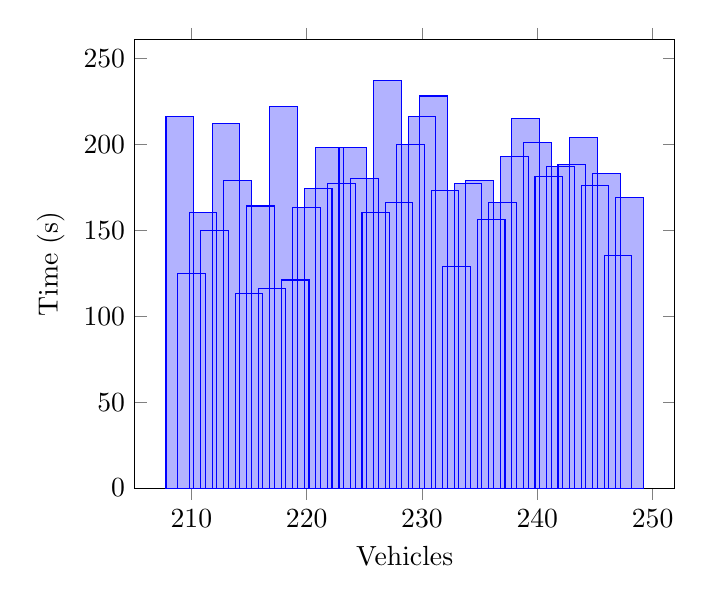
\begin{tikzpicture}
\begin{axis}[
legend style={anchor=west},
xlabel=Vehicles,
ylabel=Time (s),
ymin=0,
ybar,
]
\addplot coordinates {
(238, 193)
(239, 215)
(234, 177)
(235, 179)
(236, 156)
(237, 166)
(230, 216)
(232, 173)
(233, 129)
(245, 176)
(244, 204)
(247, 135)
(246, 183)
(241, 181)
(240, 201)
(242, 187)
(248, 169)
(209, 216)
(215, 113)
(222, 198)
(219, 121)
(214, 179)
(231, 228)
(216, 164)
(217, 116)
(212, 150)
(213, 212)
(210, 125)
(211, 160)
(218, 222)
(243, 188)
(229, 200)
(228, 166)
(227, 237)
(226, 160)
(225, 180)
(224, 198)
(223, 177)
(221, 174)
(220, 163)
};

\end{axis}
\end{tikzpicture}
\label{tik:time:0:98}
\caption{0 percent diving with GSC on route $98$}
\end{figure}
